\documentclass[11pt]{article}

\newcommand{\lectureNum}{10}
\newcommand{\lectureName}{Multi-Way Join Algorithms}
\newcommand{\lectureDate}{FIXME}

\usepackage{../dbnotes}

\begin{document}

\maketitle
\thispagestyle{plain}

%% ==================================================================
%% INTRODUCTION
%% ==================================================================
\section{Introduction}

In some cases, the intermediate result for multi-way joins might be larger than any single table, which incurs large overhead when materializing intermediate result and computing the join result. 

This is especially the case for joins with cycles in the join condition. For example,

\begin{verbatim}
SELECT * FROM R, S, T
	WHERE R.a = S.a
    AND R.b = T.a
    AND S.b = T.b;
\end{verbatim}

It is possible joining any of the two tables will produce more elements than the original table given the same join key appears multiple times in each of the table, but can be eliminated with the third join condition. To consider multiple join conditions at same time, we can use join algorithms built specifically for multi-way joins.

\subsection{Worst-Case Optimal Joins (WCOJ)}

Definition: The runtime of the join algorithm is better than all other join algorithms when the query and data represent the worst possible scenario.

This can be done by performing join by examining a variable at a time instead of a relation at a time, and therefore the runtime of a WCOJ algorithm is bounded by the output size of the result and depends on the variable evaluation ordering.

\section{Leap-Frog Trie Join}

\subsection{Common Matching}

First, we examine the algorithm to find matching keys in multiple tables\cite{veldhuizen2012leapfrog}. Assume all tables are sorted by the join key.

\begin{center}
    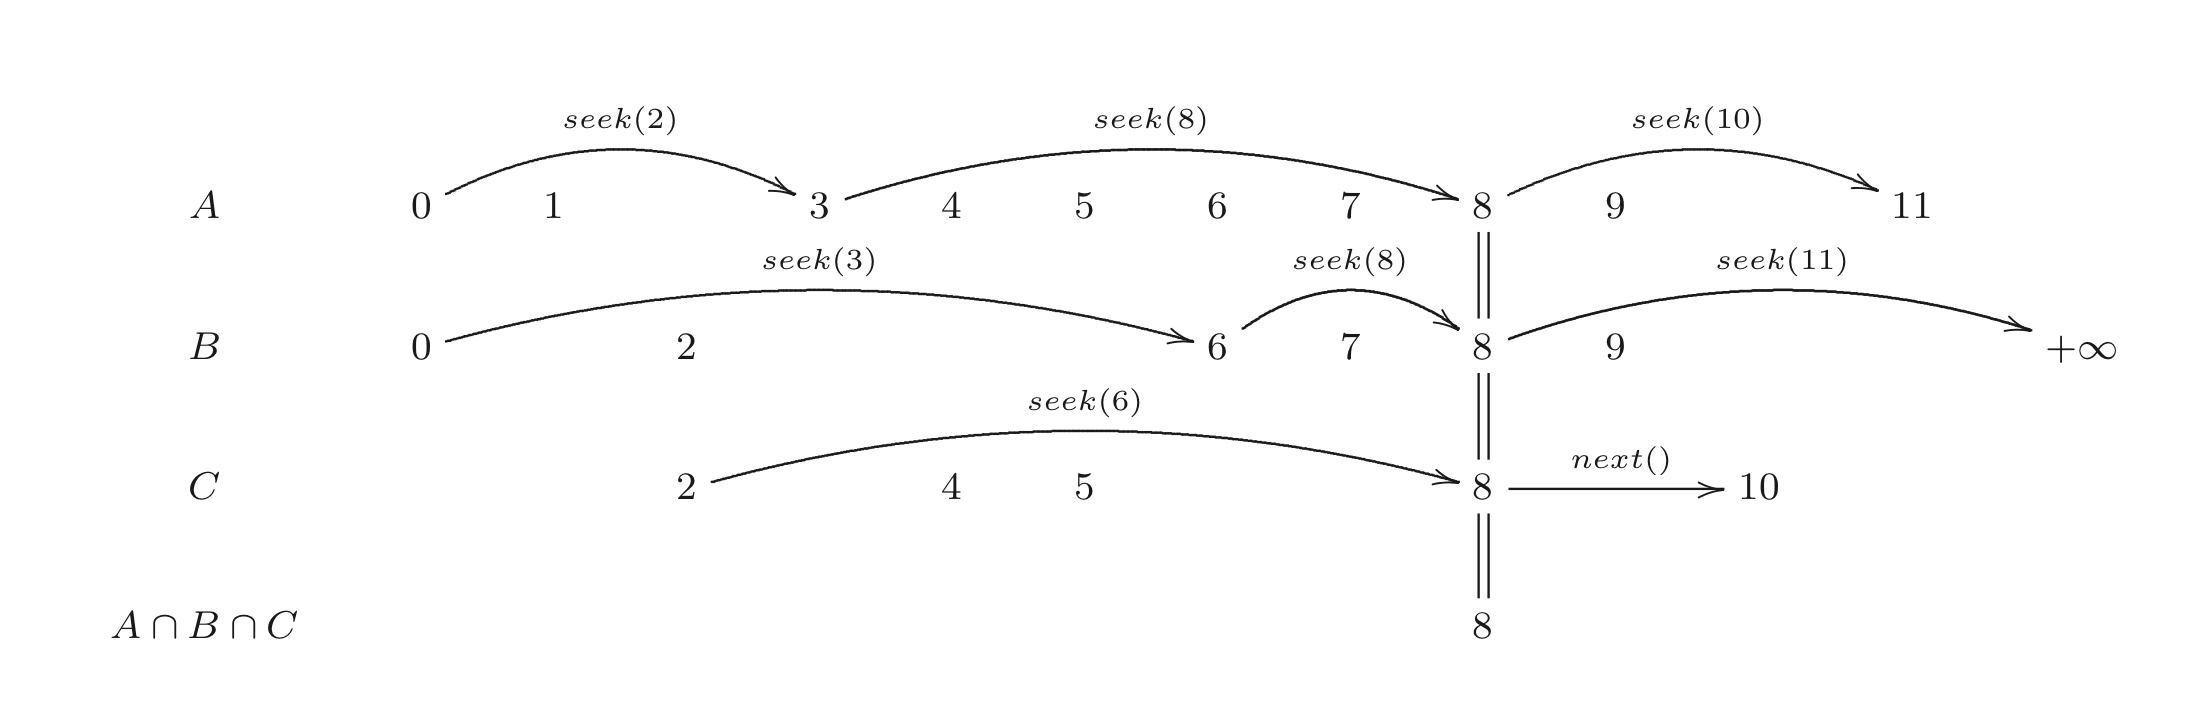
\includegraphics[width=0.8\textwidth]{img/figure1.png}
\end{center}

The algorithm assumes iterator API for the tables. Three iterators start at 0, 0, 2 respectively. And then,

\begin{itemize}
    \item Becuase C is positioned at 2, A should skip next until find the first element which is larger then or equal to 2, and it stops at 3.
    \item Given A is now at 3, we should then position B to the next key larger than or equal to 3, and it goes directly to 6.
    \item Given B is at 6, C seeks to the next position and reaches 8.
    \item Then we position A to the next position, and it also reaches 8.
    \item B also reaches 8 by advancing the iterator.
\end{itemize}

Therefore, we find the first common match 8 in the three tables.

\subsection{Multi-Join Trie}

Developed by LogicBlox in the early 2010s, leap-frog trie join builds a trie index for each relation in the join, and
each level of the trie represents a single attribute of join keys. If the table is sorted in advance, the trie index can
be built on-the-fly.

\subsection{Join Algorithm}


\begin{center}
    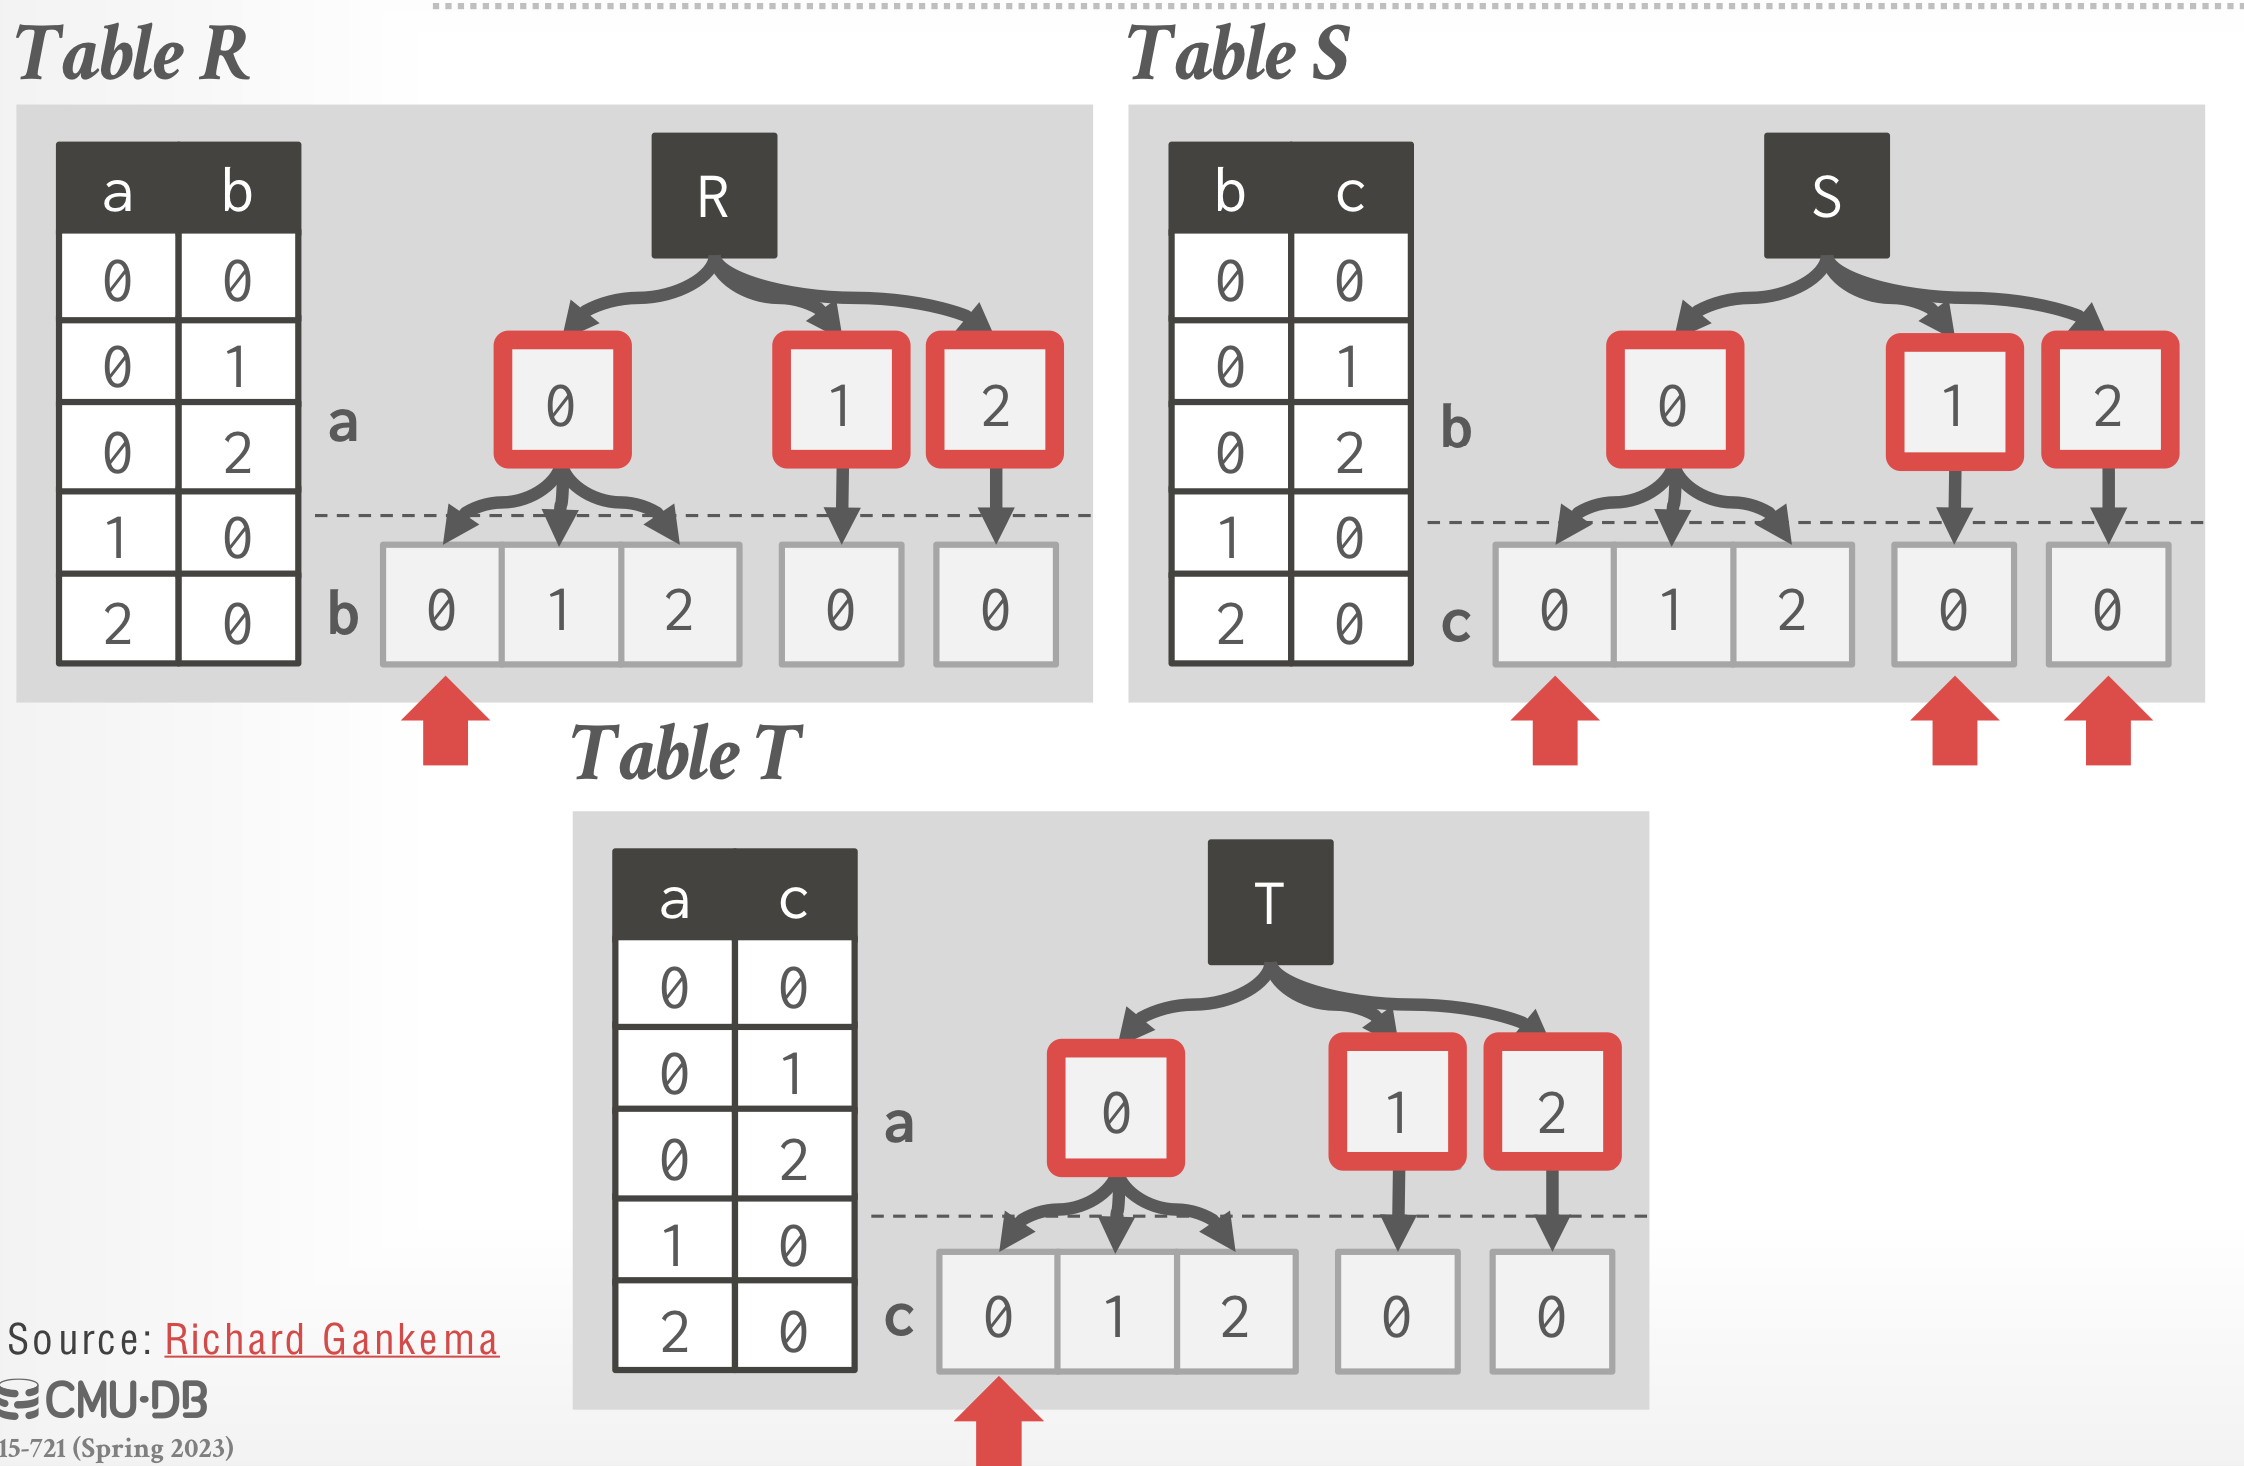
\includegraphics[width=0.8\textwidth]{img/figure2.png}
\end{center}

In order to join table R, S, T, we do the following steps:

\begin{itemize}
    \item First, we select the key a for iteration. As table R, S tries include key a, we use the matching algorithm
          described in section 1.
    \item Once we find one pair of matching key a' for key a, we then start examining the second key b in table R and S,
          using the third-layer trie of R index and second-layer trie of S index.
    \item After we find one pair of matching key b' for key b, we can then examine the third layer of trie S and the
          third layer of trie T, to obtain the matching key c' for key c.
    \item We can output (a', b', c') as one join result tuple, and repeat the process for each key.
\end{itemize}

\subsection{Observations}

Building a trie for every relation on the fly is expensive. We should build (or only part of it) only when necessary.

\section{Hash Trie Join}

\begin{center}
    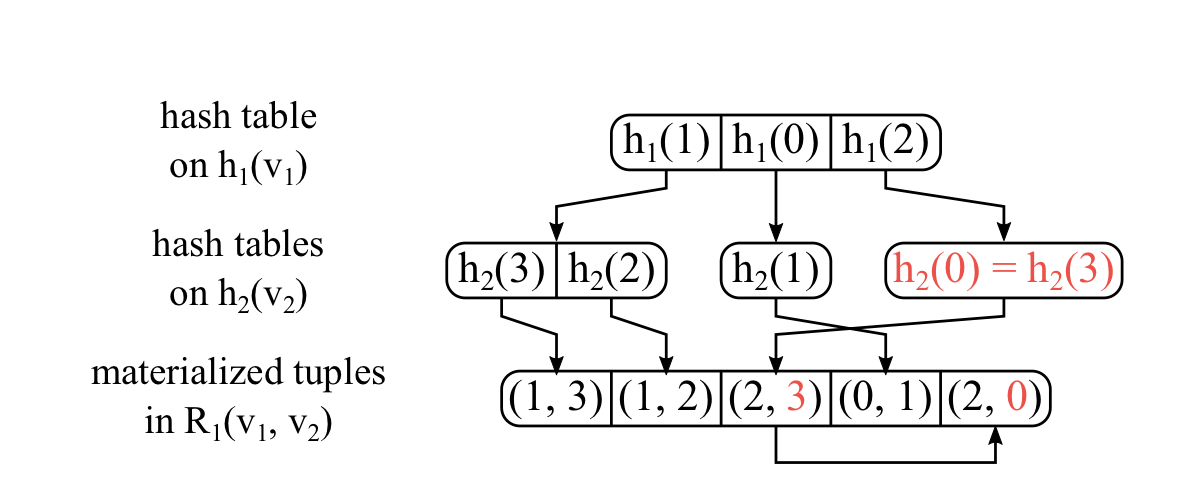
\includegraphics[width=0.5\textwidth]{img/figure3.png}
\end{center}

Instead of storing join keys in the trie, we can store the hash values in order to reduce the overhead of comparing the
full key.\cite{freitag2020adopting}

\subsection{Hash Trie}

\begin{center}
    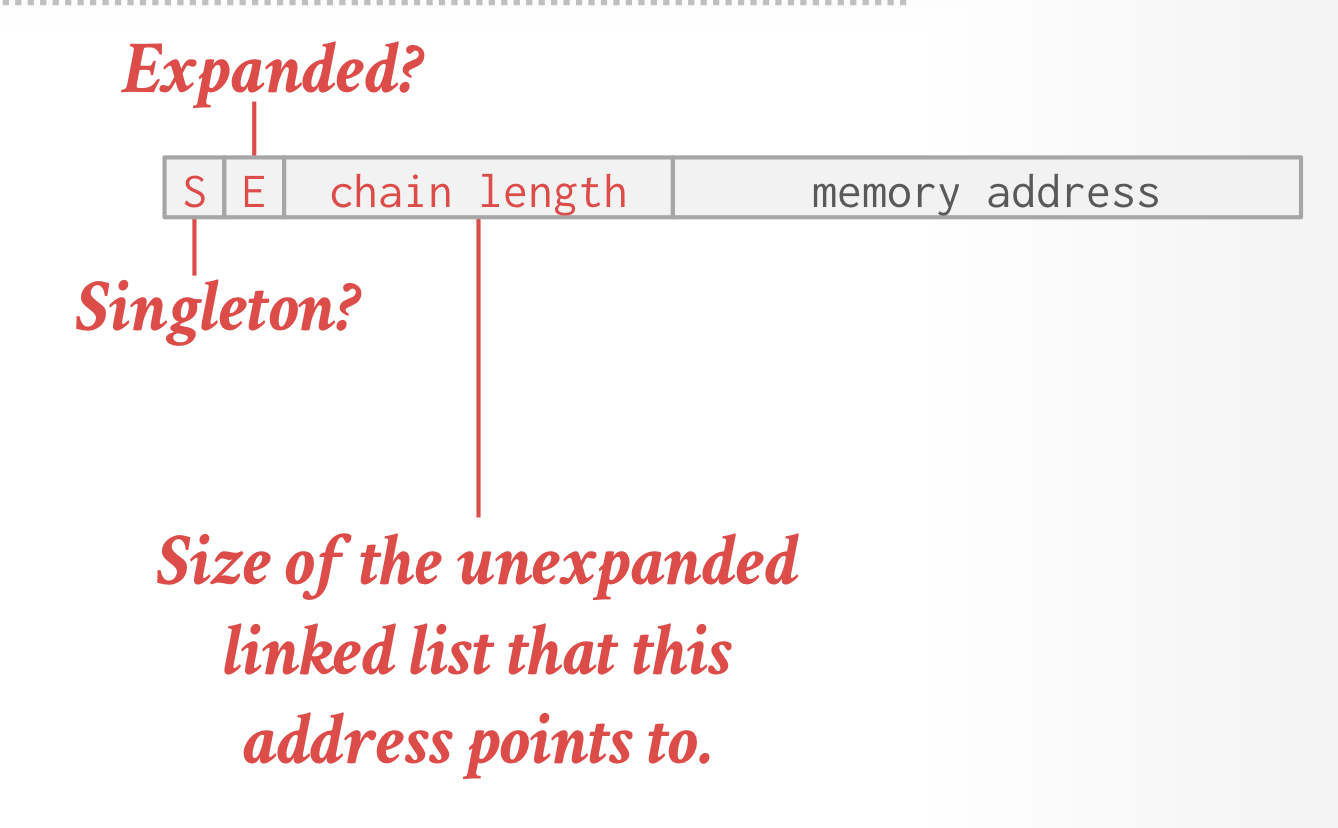
\includegraphics[width=0.8\textwidth]{img/figure4.png}
\end{center}

We can apply tagged pointer optimization to store more information within the 64-bit pointer.
For example, the hash trie implementation squashes singleton flag, expansion flag, and the chain
length into the high 16 bits of the pointer.\cite{freitag2020adopting}


\subsection{Singleton Optimization}

\begin{center}
    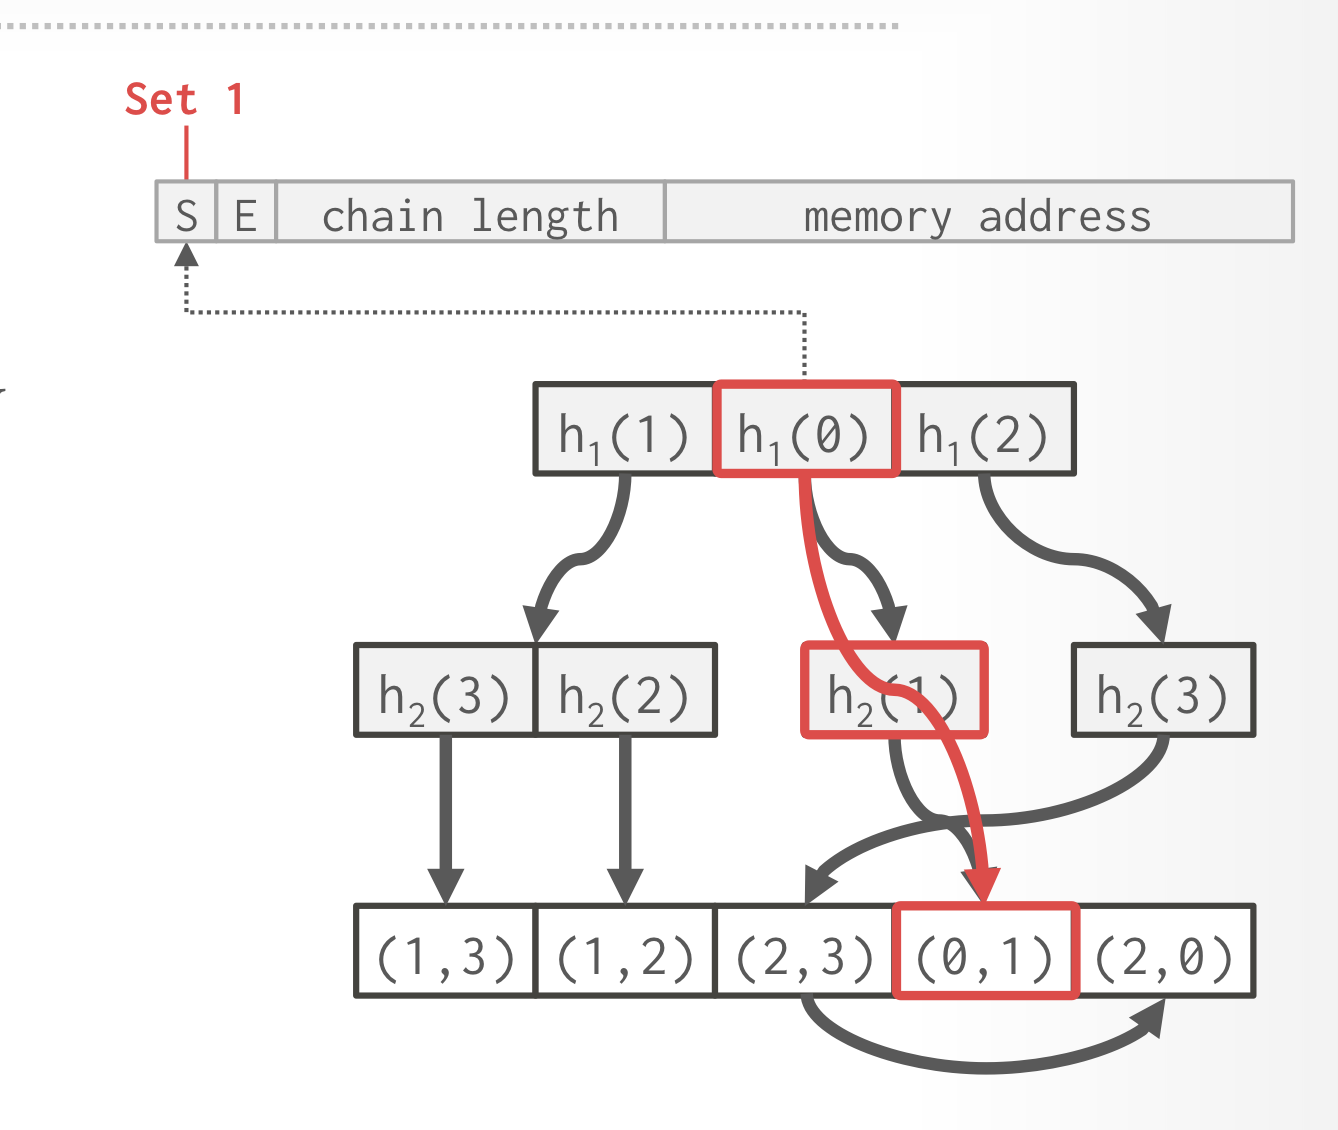
\includegraphics[width=0.5\textwidth]{img/figure5.png}
\end{center}

The lower level of the hash trie usually have fewer data. Therefore, we can directly jump to the final layer to avoid
allocating singleton nodes, as \texttt{h(0)} shown in the figure.\cite{freitag2020adopting}

\subsection{Lazy Child Expansion}


\begin{center}
    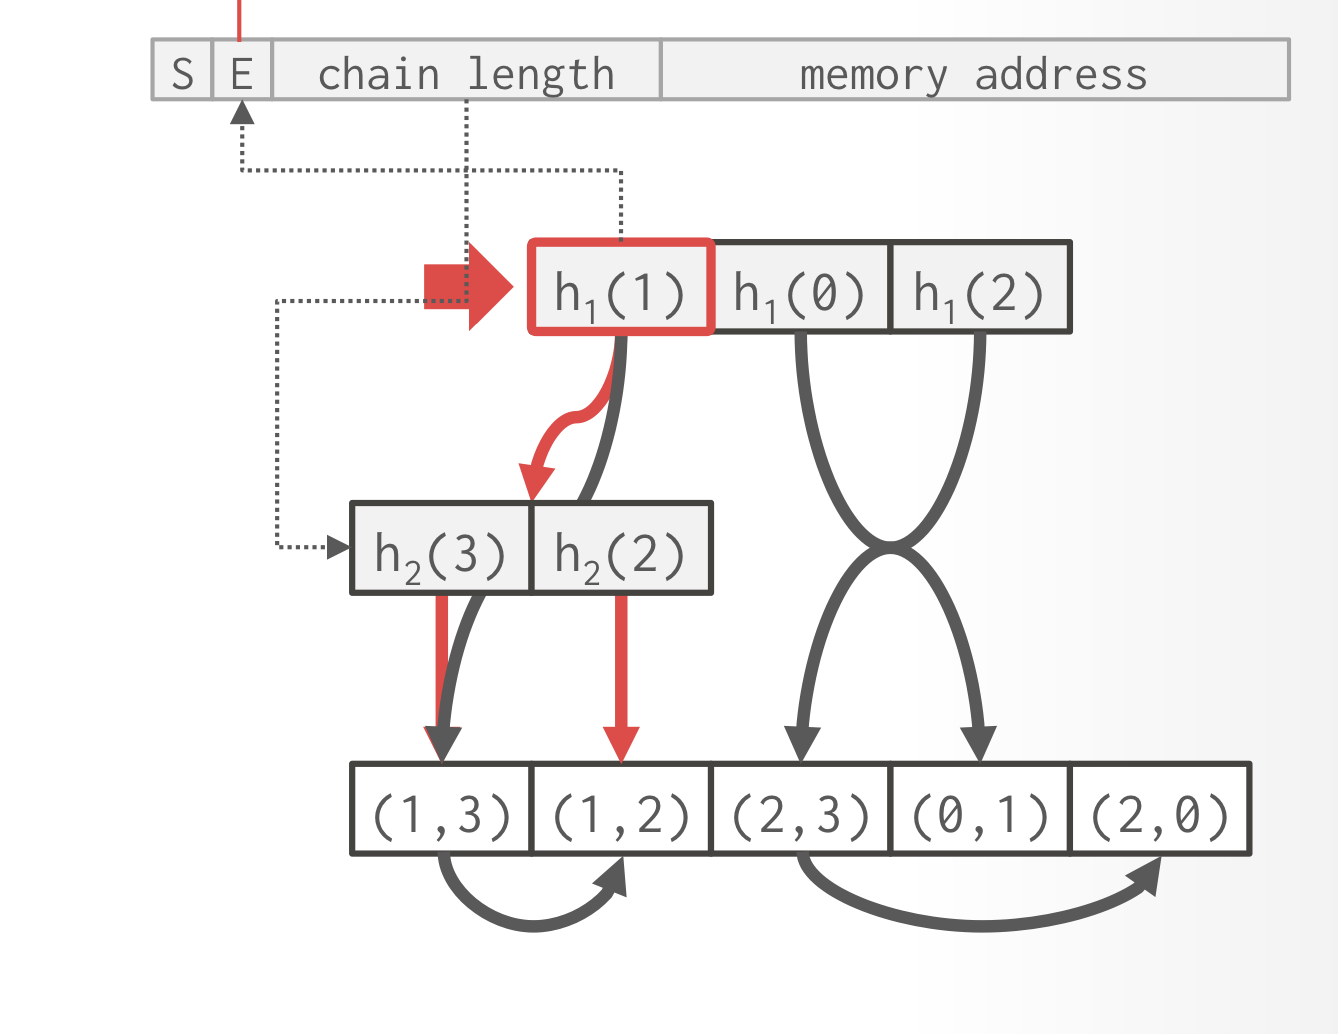
\includegraphics[width=0.5\textwidth]{img/figure6.png}
\end{center}

Some trie node may never be accessed if the filter selectivity is high. Therefore, we can only materialize inner nodes in the trie when they are accessed during the probe.\cite{freitag2020adopting}

\subsection{Optimizer Heuristics}

Multi-way joins are slower than binary joins if the query's intermediate results are not larger than its inputs.
Therefore, the optimizer needs to use heuristics to decide whether to use binary join vs. WCOJ.

% ==================================================================
% BIBLIOGRAPHY
% ==================================================================
\newpage
\bibliographystyle{abbrvnat}
\bibliography{10-multiwayjoins}

\end{document}
